\section{Supplementary Evidence}
\label{sec:supplement}

\subsection{Calibration-Derived Initial Mask}
\label{sec:init_provenance}

The GR00T initializer is produced before the full-context search. For every predeclared CKA and CS ratio, action-impact weights prioritize layers whose intervention changes the physical action output, while RMS and saturation guards keep unstable layers in FP16. A greedy byte-constrained solver and fixed-size layer flips produce nine complete candidate masks. Paired adjudication on 16 calibration observations selects one mask for each ratio without using success labels. A four-task development sweep then selects the 16:1 ratio by closed-loop macro success. This gives the fixed proxy $16(1-\widehat{\mathrm{CKA}}_i)+\widehat{D}_{\mathrm{CS},i}$ and the 100-W4/16-FP16 mask used as $M_0$.

The full-context stage is run once from the frozen $M_0$. It does not try several initial masks and retain whichever performs best. This design prevents post-hoc restarts from becoming another source of selection bias. The exact initializer artifact and its calibration buffer hash are recorded in the artifact registry. The four ratio-selection tasks are included in the 50-task aggregate. A descriptive recomputation over the other 46 tasks gives 51.8\% for ours, 27.6\% for QuantVLA W4A8, and 52.8\% for FP16. This slice is not a separately preregistered comparison, but it shows that the main pattern is not created by the four development tasks.

\subsection{Exact Metric Specification and Edge Cases}
\label{sec:metric_specification}

\paragraph{Sequence construction and action semantics.}
Each metric unit is a task--seed sequence $u$ with $R_u$ unique replans. Replans are sorted by their recorded integer index, and each contributes the complete inverse-normalized $(16,12)$ chunk executed before the next replan, giving $N_u=16R_u$. Later unexecuted forecasts are not retained, adjacent chunks do not overlap, and predictions are not deduplicated. A sequence contains only complete chunks collected before success, termination, truncation, or the official horizon. Duplicate replans, a shape other than $(16,12)$, or any non-finite value fail the metric gate rather than being padded or imputed. Coordinates 1--3 are end-effector translation, 4--6 are a rotation vector, 7 is gripper close, and 8--12 are the deployed base/control coordinates. Equation~\ref{eq:global_scale} normalizes every coordinate separately.

\paragraph{Pose map.}
For $\xi=[v;\omega]$, let $\Omega=[\omega]_{\times}$, $\theta=\lVert\omega\rVert_2$, and
\begin{equation}
\begin{aligned}
\operatorname{Exp}(\xi)
&=\begin{bmatrix}
I+A\Omega+B\Omega^2&(I+B\Omega+C\Omega^2)v\\
0&1
\end{bmatrix},\\
A&=\frac{\sin\theta}{\theta},\qquad
B=\frac{1-\cos\theta}{\theta^2},\qquad
C=\frac{\theta-\sin\theta}{\theta^3}.
\end{aligned}
\label{eq:se3_exp_detail}
\end{equation}
The implementation uses Taylor limits for $\theta<10^{-5}$. Right multiplication $T_t=T_{t-1}\operatorname{Exp}(\xi_t)$ interprets each increment in the current end-effector frame. The logarithm uses the principal rotation angle and inverse left Jacobian $V^{-1}=I-\Omega/2+c\Omega^2$, where $c=1/12$ near zero and $c=\theta^{-2}-(1+\cos\theta)/(2\theta\sin\theta)$ otherwise. The three control-specific components are
\begin{align}
 e^{\mathrm{pose}}_t&=\frac{\operatorname{Diag}(s_{1:6})^{-1}
 \operatorname{Log}((T^T_t)^{-1}T^Q_t)}{\sqrt t},\qquad
 d_{\mathrm{pose}}^{(u)}=\overline\rho_t(e^{\mathrm{pose}}_t),
 \label{eq:pose}\\
 d_{\mathrm{stitch}}&=\overline{\rho}\!\left(
 \frac{(A^Q_{r+1,1}-A^Q_{r,H})-(A^T_{r+1,1}-A^T_{r,H})}{s}
 \right),
 \label{eq:stitch}\\
 d_{\mathrm{grip}}^{(u)}&=\tfrac12\left[
 \overline\rho_t(g^Q_t-g^T_t)+
 \overline\rho_{t>1}((g^Q_t-g^Q_{t-1})-(g^T_t-g^T_{t-1}))\right],
 \label{eq:gripper}
\end{align}
where $g^P_t=\sigma(4a^P_{t,7}/s_7)$. Translation and rotation are normalized coordinatewise before averaging.

\paragraph{Functional diagnostic.}
For physical final chunks indexed by context $i$, define
\begin{equation}
\begin{aligned}
 e_i&=\frac{\lVert A_i^Q-A_i^T\rVert_F^2}
 {\max(\lVert A_i^T\rVert_F^2,10^{-8})},\qquad
 d_{\mathrm{final}}=\frac{\lVert A^Q-A^T\rVert_F^2}
 {\max(\lVert A^T\rVert_F^2,10^{-8})},\\
 \dfunc&=d_{\mathrm{final}}+d_{\mathrm{kin}}+d_{\mathrm{grip}}
 +2\operatorname{CVaR}_{0.9}(d_{\mathrm{solver}}).
\end{aligned}
\label{eq:dfunc_detail}
\end{equation}
$d_{\mathrm{kin}}$ is one half the sum of the analogous relative errors restricted to translation and rotation coordinates; $d_{\mathrm{solver}}=\operatorname{mean}_i e_i$, and $\operatorname{CVaR}_{0.9}$ averages the $e_i$ values at or above their empirical 90th percentile. The registered \dfunc gripper term is the fraction of adjacent solver states whose active gripper changes ($>10^{-4}$ in both policies) disagree in sign. The shared selection path records only final physical chunks and no internal solver trajectory, so this legacy \dfunc gripper term is zero there; gripper deviation still enters \dpac through Equation~\ref{eq:gripper} and the explicit component guard.

\paragraph{Evaluation order.}
For each candidate, we (1) validate paired records, sort replans, and inverse-normalize final chunks; (2) compute the global 12-coordinate scale once from all FP16 selection chunks; (3) evaluate Equations~\ref{eq:local_prefix}, \ref{eq:pose}, \ref{eq:stitch}, and \ref{eq:gripper} per task--seed sequence; (4) form the five-component mean and worst-10\% sequence mean in Equation~\ref{eq:dpac_sequence}; and (5) compute task-level candidate-minus-$M_0$ differences, leave-one-task-out standard errors, $J$, and the pose/stitch/gripper upper bounds. A one-replan sequence has $d_{\mathrm{stitch}}=0$, while a one-action sequence has a zero gripper-difference term. Acceptance requires strict $J_{\mathrm{final}}<0$, non-positive component upper bounds, and the exact byte constraint; equality fails closed.

\subsection{Frozen GR00T Decision Record}

The GR00T search starts from the frozen $M_0$. All 116 valid one-layer flips have non-positive benefit under the cross-context score. The additive dynamic program therefore emits no beneficial half- or full-budget combination. Five additional structured proposals are evaluated as complete networks; every alternative has a positive paired minimax objective or violates a pose, stitch, or gripper deviation guard. The fail-closed output is unchanged $M_0$. These facts record rejection only within $\mathcal C(M_0)$ and do not establish local optimality outside that finite class.

The final plan uses signed-nibble group-64 weights, identity row rotation, per-forward dynamic A8, and no ATM, OHB, error-folding, calibration bypass, or runtime selector. Its SHA-256 is recorded in the artifact registry and checked before table generation.

\subsection{Mask Diagnostic Robustness}
\label{sec:mask_diagnostic}

The registered 50-episode diagnostic compares $M_0$ with uniform full-W4 under an otherwise identical runtime. $M_0$ obtains 56\% versus 46\%, with ten paired wins, five losses, and 35 ties ($p=0.302$). An earlier 50-episode exploratory wave reverses direction (50\% versus 52\%); pooling both waves gives 53\% versus 49\% ($p=0.557$). The diagnostic is therefore disclosed only as a robustness check and does not support a causal claim or enter the headline evaluation.

\subsection{Paired Statistical Detail}

Against QuantVLA W4A8, 1,647 of 2,500 episodes are tied, 721 favor ours, and 132 favor QuantVLA. Exact two-sided McNemar testing gives $p=6.30\times10^{-99}$. Holm adjustment over the registered comparison family gives $p=1.89\times10^{-98}$. Against FP16, the corresponding counts are 1,889 ties, 292 wins, and 319 losses, with $p=0.2929$.

\subsection{Reduced Closed-Loop Component Ablation}
\label{sec:component_rollout_detail}

The component study uses all 50 tasks and ten paired seeds per task. It is disjoint from mask construction and was aggregated only after all 1,500 new episodes passed the coverage audit. The matched $M_0$ reference obtains 73.9\%, 46.9\%, and 38.1\% on Atomic-Seen, Composite-Seen, and Composite-Unseen, respectively. Its overall success rate is 53.8\%.

Frozen-range A8 obtains 0.0\% on every split. All 500 episodes complete normally, with no crash or numerical-failure row. Relative to $M_0$, it has no paired wins, 269 losses, and 231 ties. The Holm-adjusted McNemar value is $6.33\times10^{-81}$. This result is specific to the frozen table constructed under our calibration protocol and is not a claim that every static activation quantizer must fail.

Local-MSE selection obtains 72.8\%, 43.8\%, and 40.0\% across the three splits, for 53.0\% overall. It has 55 paired wins, 59 losses, and 386 ties against $M_0$. The no-final-check proposal obtains 70.6\%, 38.8\%, and 47.5\%, also giving 53.0\% overall. It has 54 wins, 58 losses, and 388 ties. Both Holm-adjusted values are 1.0. The split reversal for the no-final-check proposal illustrates why the full 50-task result is preferable to conclusions drawn from only the two seen groups. Neither non-significant comparison is treated as evidence of equivalence.

\subsection{Dynamic-Range Evidence}
\label{sec:dynamic_range_visualization}

\begin{figure}[t]
  \centering
  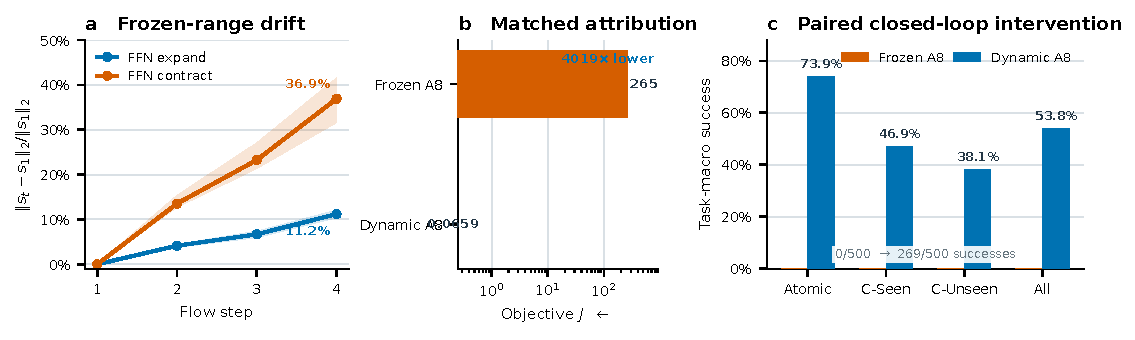
\includegraphics[width=\textwidth]{figures/dypac_dynamic_range_evidence.pdf}
  \caption{Evidence for per-forward A8 scaling. \textbf{(a)} Calibrated per-channel ranges drift across flow steps. \textbf{(b)} Matched offline attribution relative to A16 under objective $J$ (log scale). \textbf{(c)} Under an otherwise identical $M_0$ runtime, the registered static table obtains 0/500 successes and dynamic A8 obtains 269/500. The intervention evaluates this specific static construction, not every possible static activation quantizer.}
  \label{fig:dynamic_range_evidence}
\end{figure}


Figure~\ref{fig:dynamic_range_evidence} separates mechanism diagnosis from behavioral evidence. Across the 31 applicable action-head layers, the median scale drift is 10.8\%, 16.8\%, and 24.9\% at flow steps 2--4, and the maximum layer-step value is 49.0\%. These frozen-table statistics do not by themselves establish a success effect. The matched offline attribution reduces $J$ from 467.52 to 0.518, while the paired closed-loop intervention compares 0/500 successes for the registered static table with 269/500 for per-forward dynamic A8 under the otherwise identical $M_0$ runtime.

\subsection{Full-Policy Audit Outcome}
\label{sec:fcp_visualization}

\begin{figure}[ht]
  \centering
  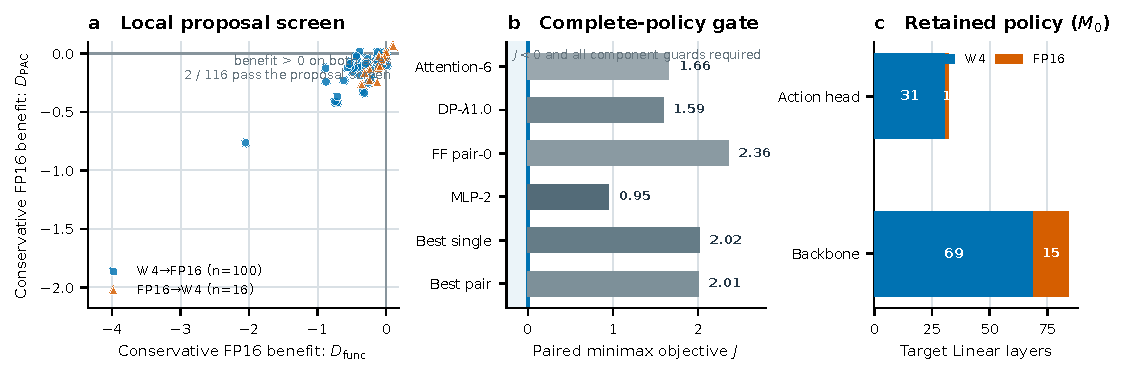
\includegraphics[width=\textwidth]{figures/dypac_fcp_audit.pdf}
  \caption{GR00T deviation-based decision record with corrected task-level statistics. \textbf{(a)} Two of 116 coordinates have positive conservative benefit for retaining FP16 under both metrics. Both are already protected; these are not two improving removals. \textbf{(b)} All six rebuilt complete-policy candidates have $J>0$ and fail a component guard. \textbf{(c)} The 100-W4/16-FP16 initializer is retained. This decision does not establish its success optimality or demonstrate an effect of candidate-state adjudication, which was not triggered.}
  \label{fig:fcp_audit}
\end{figure}

Figure~\ref{fig:fcp_audit} makes the acceptance boundary explicit. Every valid one-layer precision flip has non-positive conservative benefit under both \dfunc and \dpac. All five complete structured proposals also have positive minimax objective ($J=3.97$--$6.87$) and fail the registered component-deviation gate. The full-policy audit consequently abstains and returns the unchanged 100-W4/16-FP16 $M_0$. This visualization documents the decision only within the declared search neighborhood; no separate gain or global-optimality claim follows from it.

\subsection{Storage Accounting}

The GR00T FP16 static-component scope is 2,139,537,408 bytes. The final plan occupies 962,068,480 bytes, including 327,352,320 fixed bytes and packed mixed-precision target components, for 2.2239$\times$ compression. This is 0.9982$\times$ the QuantVLA cell of 963,772,416 bytes and satisfies the preregistered 1.10$\times$ ceiling. The $\pi_{0.5}$ FP16 scope is 4,416,602,112 bytes. Its 1,634,828,288-byte plan gives 2.7016$\times$ compression.

These values are static packed estimates. Activations, CUDA workspaces, simulator state, and eager fake-quant caches are outside the scope. Therefore no runtime speed or peak-memory conclusion follows from the compression ratios.

\subsection{$\pi_{0.5}$ Formal Result}

The $\pi_{0.5}$ transfer uses four flow steps on the complete RoboCasa365 target split, matching the completed reference rows, with 50 seeds on each of 50 tasks. The 121-W4/59-FP16 policy completes all 2,500 episodes without a missing, duplicate, or failed row. It records 536/900 Atomic-Seen, 123/800 Composite-Seen, and 34/800 Composite-Unseen successes, giving 693/2,500 overall. The corresponding task-macro rates are 59.6\%, 15.4\%, 4.3\%, and 27.7\% overall. The result supports a formal success--storage operating point at 1,634,828,288 bytes and 2.702$\times$ compression. Cross-row differences remain descriptive because this experiment does not register a paired significance comparison with the other $\pi_{0.5}$ configurations.

\subsection{Extended Ablation Protocol}
\label{sec:extended_ablations}

Table~\ref{tab:extended_ablation_plan} registers the experiments needed to test claims that the completed evidence does not support. Every selection experiment will start from frozen checkpoints and manifests, preserve exact-byte accounting, report the resulting mask rather than force equal layer counts, and use paired task--seed evaluation. All entries remain pending and contribute no numerical evidence to the current paper.

\begin{table}[h!]
\centering
\caption{Registered pending experiments. These studies are not complete and provide no numerical evidence in the current paper.}
\label{tab:extended_ablation_plan}
\small
\setlength{\tabcolsep}{4.0pt}
\renewcommand{\arraystretch}{1.08}
\begin{tabular}{@{}p{0.17\linewidth}p{0.39\linewidth}p{0.25\linewidth}p{0.10\linewidth}@{}}
\toprule
Family & Variants & Controlled readout & Status \\
\midrule
Full-policy audit behavior & Multiple initial masks and byte budgets; compare accepted masks with their initializers & Acceptance/abstention rate; paired success and byte deltas & Pending \\
\dpac predictive validity & Rank a broad library of masks and activation variants using \dpac, \dfunc, and MSE & Spearman/Kendall correlation with rollout success & Pending \\
\dpac components & Remove prefix, pose, stitch, gripper, or CVaR one at a time & Rank stability, selected mask, paired success & Pending \\
Static A8 controls & Max, clipped percentile, per-flow, and sequence-aware static calibration & Paired success, objective, saturation rate & Pending \\
$\pi_{0.5}$ paired inference & Register the four-flow-step Ours--reference paired comparison family & Exact McNemar, Holm correction, and task-level deltas & Pending \\
QVLA/ActQuant extension & Complete the registered GR00T and $\pi_{0.5}$ formal rows & Coverage audit, task-macro success, exact bytes & Pending \\
Guard validation & Relate pose, stitch, and gripper deviation bounds to observed control failures & Calibration/AUROC; failure-category rates & Pending \\
Budget sensitivity & $1.00$, $1.05$, and $1.10\times$ the QuantVLA static-byte cell & Independently selected success--storage points & Pending \\
\bottomrule
\end{tabular}
\vspace{2pt}
\parbox{0.99\textwidth}{\footnotesize Each row is a protocol commitment rather than a result. \emph{Pending} means that no value from the experiment is used in the Abstract, main claims, or statistical comparisons. The guard-validation row evaluates surrogate control deviations and is not a physical-safety certification protocol.}
\end{table}


\clearpage
\subsection{Protocol-Registered LIBERO Extension}
\label{sec:libero_comparison}

\begin{table}[H]
\centering
\caption{LIBERO: \method averages 97.3\% on $\pi_{0.5}$ and 93.8\% on GR00T.}
\label{tab:omega_qvla_libero}
\footnotesize
\setlength{\tabcolsep}{4.2pt}
\renewcommand{\arraystretch}{0.92}
\begin{tabular}{@{}lrrrrrr@{}}
\toprule
Configuration & Goal $\uparrow$ & Spatial $\uparrow$ & Object $\uparrow$ & Long $\uparrow$ & Avg. $\uparrow$ & \shortstack{Size\\(GiB) $\downarrow$} \\
\midrule
\multicolumn{7}{@{}l}{\textbf{$\pi_{0.5}$}} \\
\quad FP16 & 95.0 & 100.0 & 98.0 & 94.0 & 96.8 & 4.113 \\
\quad \quantvla W4A8 & 97.0 & 97.0 & 98.0 & 93.0 & 96.3 & 1.388 \\
\quad Uniform W6 & 99.0 & 97.0 & 99.0 & 92.0 & 96.8 & 1.902 \\
\quad $\Omega$-QVLA W4A4 & 100.0 & 99.0 & 97.0 & 96.0 & 98.0 & 1.307 \\
\quad QVLA (4.0 BPW)$^{\dagger}$ & 96.4 & 98.0 & 97.2 & 91.8 & 95.8 & 2.7 \\
\quad ActQuant (4.0 BPW)$^{\dagger}$ & 96.8 & 98.4 & 99.4 & 91.8 & 96.6 & 2.7 \\
\quad \textbf{\method (Ours)} & 99.0 & 100.0 & 96.0 & 94.0 & 97.3 & 1.788 \\
\bottomrule
\end{tabular}
\end{table}
\begin{table}[H]
\centering
\addtocounter{table}{-1}
\renewcommand{\theHtable}{\arabic{table}b}
\caption{LIBERO results (continued): GR00T N1.5.}
\footnotesize
\setlength{\tabcolsep}{4.2pt}
\renewcommand{\arraystretch}{0.92}
\begin{tabular}{@{}lrrrrrr@{}}
\toprule
Configuration & Goal $\uparrow$ & Spatial $\uparrow$ & Object $\uparrow$ & Long $\uparrow$ & Avg. $\uparrow$ & \shortstack{Size\\(GiB) $\downarrow$} \\
\midrule
\multicolumn{7}{@{}l}{\textbf{GR00T N1.5}} \\
\quad FP16 & 88.0 & 87.0 & 96.0 & 76.0 & 86.8 & 1.993 \\
\quad \quantvla W4A8 & 89.0 & 85.0 & 79.0 & 72.0 & 81.3 & 0.898 \\
\quad Uniform W6 & 85.0 & 83.0 & 92.0 & 22.0 & 70.5 & 1.109 \\
\quad $\Omega$-QVLA W4A4 & 87.0 & 86.0 & 89.0 & 76.0 & 84.5 & 0.599 \\
\quad \textbf{\method (Ours)} & 97.0 & 95.0 & 98.0 & 85.0 & 93.8 & 0.948 \\
\bottomrule
\end{tabular}
\vspace{2pt}
\parbox{0.99\textwidth}{\footnotesize The complete local matrix contains 4,000 episodes across 40/40 exact-valid cells. Each local suite uses ten tasks and ten held-out initial states. Size includes packed weights and metadata and is averaged over suite-specific masks. $^{\dagger}$The $\pi_{0.5}$ QVLA and ActQuant rows are source-reported 4.0-BPW results~\cite{akbari2026actquant} using the source memory definition.}
\end{table}


Table~\ref{tab:omega_qvla_libero} extends rather than defines the central claim. The corrected GR00T \method row obtains 97.0\%, 95.0\%, 98.0\%, and 85.0\% on Goal, Spatial, Object, and Long (93.8\% average). Each local cell contains 100 episodes over ten tasks and held-out initial states 10--19; all 40 cells pass the joint gate, for 4,000 episodes with no missing or duplicate keys. The rerun executes five actions per replan with paired action noise. We report the corrected measurement without treating the change from the invalid run as an algorithmic gain.

On GR00T, \quantvla W4A8, Uniform W6, and $\Omega$-QVLA W4A4 average 81.3\%, 70.5\%, and 84.5\%, versus 86.8\% for FP16. On $\pi_{0.5}$, the corresponding local low-bit rows average 96.3\%, 96.8\%, and 98.0\%. Tightly packed static size is reported for every local row. The two 4.0-BPW $\pi_{0.5}$ anchors from ActQuant~\cite{akbari2026actquant} are source-reported; its QVLA row reproduces QVLA~\cite{xu2026qvla} under the same 60-episode calibration budget. Neither enters local coverage, and their 2.7-GB cells are not compared with locally audited size.
